\chapter{Timeplan}
\label{cha:timeplan}

%\begin{itemize}
%\item Include a gantt chart here (do it with MS Visio or Excel),
%it should have about 10 tasks clustered into about 4 groups:
%literature study, design, implementation, evaluation.
%\item Give a brief explanation of the timeplan.
%\end{itemize}
The time plan as shown in figure \ref{fig:labelOfThesisTimePlan} is to achieve the goals of this thesis. The thesis will be structured into the following way:
\begin{itemize}
	\item Literature review is one of the important activities of the thesis. It will be carried out till selecting the dimensionality reduction algorithm.
	\item Analysis of the state-on-algorithm will be done with the progress of the literature review.
	\item We need to select the high dimensional dataset. Its better to find the data from streaming sources but high dimensional data from static souce will also be fine. The dataset is selected in November but the dataset may be modified or new dataset can be added with the progress of the thesis. 
	\item There will be more than one tasks to implement the framework. If the dataset is static then we need to implement it to convert stream dataset. Implementation of the incremental Linear Discriminant Analysis is the main task of the thesis. In this thesis, a fast, scalable framework should be developed for the streaming data. This will be continued with the parallel of other tasks of the thesis but it will be in main focus from December to February.
	\item Evaluation is another big topic for this thesis.The evaluation will be done after the implementation in March.
	\item Thesis writing will be done through out the whole time of the thesis and preparation for the presentation will be done at the last month of thesis.
\end{itemize}

\begin{figure}[htbp]
	% center the image.
	\centering
	
	% include a png file. Adapt size to 0.5 * textwidth and retain aspect ratio (!)
	\resizebox{\textwidth}{!}{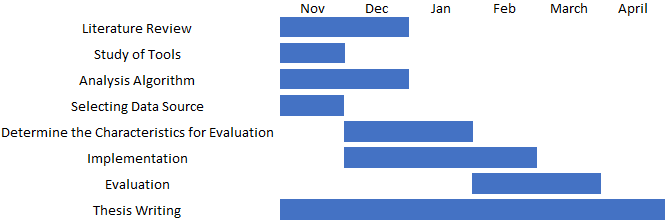
\includegraphics{Thesis_Time_Plan.png}}
	
	\caption{Thesis Time Plan}
	\label{fig:labelOfThesisTimePlan}
\end{figure}
In fig \ref{fig:labelOfThesisImplementation} the details of implementation is given. The Implementation is started by designing the framework and finished with the completion of task reduced dimensionality visualization with evaluation information. In time plan, we mentioned the implementation will be from December to March. In this diagram, we will show the individual task started from which date and finished on which date. This will help to implement the thesis in a planed, structured way.\\\\
The design of the framework is required for 10 days. The presentation layer is for 7 days. We will implement the access layer in one week. The Business layer is required to 7 weeks to finish.  
\begin{figure}[htbp]
	% center the image.
	\centering
	
	% include a png file. Adapt size to 0.5 * textwidth and retain aspect ratio (!)
	\resizebox{\textwidth}{!}{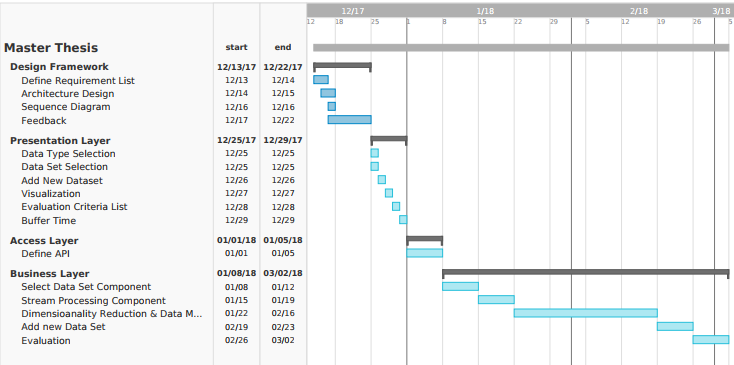
\includegraphics{Break_Down_Implementation.png}}
	
	\caption{Details of Implementation}
	\label{fig:labelOfThesisImplementation}
\end{figure}